\begin{frame}{Trasmettere funzioni}
	\vspace{-0.8cm}
	\begin{figure}
		\centering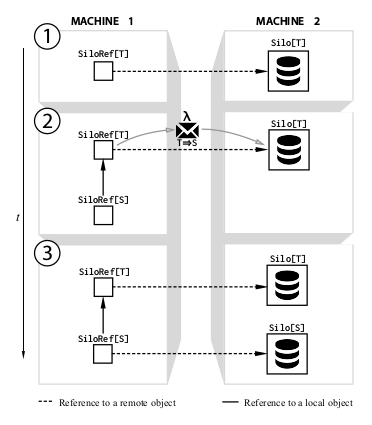
\includegraphics[scale=0.5]{functionPassing}
	\end{figure}
	\begin{tikzpicture}[remember picture,overlay]
	\node<2>[draw,minimum size=1.2cm,line width=1pt,red,circle] at (7.2,7) {};
	\node<3>[draw,minimum size=1.2cm,line width=1pt,red,circle] at (3.9,7) {};
	\node<4>[draw,minimum size=1.2cm,line width=1pt,red,circle] at (5.4,5.8) {};
	\end{tikzpicture}
\end{frame}